\documentclass[12pt, a4paper, oneside]{ctexart}
\usepackage{amsmath, amsthm, amssymb, bm, color, graphicx, geometry, mathrsfs,extarrows, braket, booktabs, array, xcolor, fontspec, appendix, float, subfigure, wrapfig}
\usepackage[colorlinks,linkcolor=red,anchorcolor=blue,citecolor=blue,urlcolor=blue,menucolor=black]{hyperref}

%%%% 设置中文字体 %%%%
\setCJKmainfont{方正新书宋_GBK.ttf}[ BoldFont = 方正小标宋_GBK, ItalicFont = 方正楷体_GBK]
%%%% 设置英文字体 %%%%
\setmainfont{Times New Roman}
\setsansfont{Calibri}
\setmonofont{Consolas}

%%%% 设置代码块 %%%%
% 在vscode中使用minted需要先配置python解释器, Ctrl+Shift+P, 输入Python: Select Interpreter选择安装了Pygments的Python版本. 再在setting.json中xelatex和pdflatex的参数中加入 "--shell-escape", 即可
% TeXworks中配置方法参考: https://blog.csdn.net/RobertChenGuangzhi/article/details/108140093
\usepackage{minted}
\renewcommand{\theFancyVerbLine}{
    \sffamily\textcolor[rgb]{0.5,0.5,0.5}{\scriptsize\arabic{FancyVerbLine}}} % 修改代码前序号大小
\newmintinline{cpp}{linenos, breaklines, frame=lines}  % 使用\cppinline{代码}
\newminted{cpp}{linenos, breaklines, frame=lines}  % 使用\begin{cppcode}代码\end{cppcode}
\newmintinline{python}{linenos, breaklines, frame=lines, python3}  % 使用\pythoninline{代码}
\newminted{python}{linenos, breaklines, frame=lines, python3}  % 使用\begin{pythoncode}代码\end{pythoncode}
\newmintedfile{python}{linenos, breaklines, frame=lines, python3}  % 使用\pythonfile{代码地址}

%%%% 设置行间距与页边距 %%%%
\linespread{1.2}
\geometry{left=2.5cm, right=2.5cm, top=2.5cm, bottom=2.5cm}

%%%% 定理类环境的定义 %%%%
\newtheorem{example}{例}            % 整体编号
\newtheorem{theorem}{定理}[section] % 定理按section编号
\newtheorem{definition}{定义}
\newtheorem{axiom}{公理}
\newtheorem{property}{性质}
\newtheorem{proposition}{命题}
\newtheorem{lemma}{引理}
\newtheorem{corollary}{推论}
\newtheorem{remark}{注解}
\newtheorem{condition}{条件}
\newtheorem{conclusion}{结论}
\newtheorem{assumption}{假设}
\numberwithin{equation}{section}  % 公式按section编号 (公式右端的小括号)
\newtheorem{algorithm}{算法}
\newsavebox{\nameinfo}
\renewenvironment{title}[1]{
    \sbox{\nameinfo}{\zihao{4} #1}
    \begin{center}
    \zihao{-2}\bf
}{\vspace{-0.2cm}\\\usebox{\nameinfo}\end{center}}  % \begin{title}{作者信息}

%%%% 图片相对路径 %%%%
\graphicspath{{figure/}} % 当前目录下的figure文件夹, {../figure/}则是父目录的figure文件夹
\setlength{\abovecaptionskip}{-0.2cm}  % 缩紧图片标题与图片之间的距离
\setlength{\belowcaptionskip}{0pt} 

\everymath{\displaystyle} % 默认全部行间公式, 想要变回行内公式使用\textstyle
\DeclareMathOperator*\uplim{\overline{lim}}     % 定义上极限 \uplim_{}
\DeclareMathOperator*\lowlim{\underline{lim}}   % 定义下极限 \lowlim_{}
\DeclareMathOperator*{\argmax}{arg\,max}  % \argmin
\DeclareMathOperator*{\argmin}{arg\,min}  % \argmax
\let\leq=\leqslant % 简写小于等于\leq (将全部leq变为leqslant)
\let\geq=\geqslant % 简写大于等于\geq (将全部geq变为geqslant)

%%%% 一些宏定义 %%%%%
\def\bd{\boldsymbol}        % 加粗(向量) boldsymbol
\def\disp{\displaystyle}    % 使用行间公式 displaystyle(默认)
\def\tsty{\textstyle}       % 使用行内公式 textstyle
\def\sign{\text{sign}}      % sign function
\def\wtd{\widetilde}        % 宽波浪线 widetilde
\def\R{\mathbb{R}}          % Real number
\def\C{\mathbb{C}}          % Complex number
\def\Q{\mathbb{Q}}          % Rational number
\def\N{\mathbb{N}}          % Natural number
\def\Z{\mathbb{Z}}          % Integer number
\def\d{\mathrm{d}}          % differential operator
\def\e{\mathrm{e}}          % Euler's number
\def\i{\mathrm{i}}          % imaginary number
\def\re{\mathrm{Re}}        % Real part
\def\im{\mathrm{Im}}        % Imaginary part
\def\L{\mathcal{L}}         % Loss function
\def\wdh{\widehat}          % 宽帽子 widehat
\def\ol{\overline}          % 上横线 overline
\def\ul{\underline}         % 下横线 underline
\def\add{\vspace{1ex}}      % 增加行间距
\def\del{\vspace{-1.5ex}}   % 减少行间距

%%%% 正文开始 %%%%
\begin{document}
\begin{title}{强基数学002\quad 吴天阳\quad 2204210460}
    CVPR第二次作业
\end{title}
% \setcounter{section}{1}
\section{实验目的}
1. 完成图像的几何变换实验,包括:平移变换;旋转变换;欧式变换;相似变换;仿射变换.

2. 完成图像的高斯金字塔表示与拉普拉斯金字塔表示,讨论前置低通滤波与抽样频率的关系.

3. 基于高斯一阶微分的图像梯度(幅值图与方向图),分析高斯方差对图像梯度的影响.

4. 掌握Canny边缘检测原理,完成图像的边缘检测实验,展示每个环节的处理结果(梯度图、NMS、边缘链接).

5. 掌握Harris角点检测原理,完成图像的角点检测实验,分析窗⼝参数对角点检测的影响,讨论角点检测的不变.
\section{实验原理}
\subsection{图像参数化几何变换原理}
1. 平移变换(自由度为$2$)
\begin{equation*}
    \bd{x}' = \bd{x}+\bd{t}\iff \bd{x}' = \left[\begin{matrix}
        1&0&t_1\\ 0&1&t_2\\ 0&0&1
    \end{matrix}\right]\left[\begin{matrix}
        x_1\\x_2\\1
    \end{matrix}\right],\ \text{逆矩阵为}\ \left[\begin{matrix}
        1&0&-t1\\0&1&-t2\\0&0&1
    \end{matrix}\right].
\end{equation*}

2. 旋转变换(自由度为$1$)
\begin{equation*}
    \bd{x}' = R_{\theta}\bd{x}\iff \bd{x}' = \left[\begin{matrix}
        \cos\theta&-\sin\theta&0\\
        \sin\theta&\cos\theta&0\\
        0&0&1
    \end{matrix}\right]\left[\begin{matrix}
        x_1\\x_2\\1
    \end{matrix}\right],\ \text{逆矩阵为}\ \left[\begin{matrix}
        \cos\theta&\sin\theta&0\\
        -\sin\theta&\cos\theta&0\\
        0&0&1
    \end{matrix}\right].
\end{equation*}

3. 欧式变化(自由度为$3$)
\begin{equation*}
    \bd{x}' = [R_\theta|\bd{t}]\bd{x}\iff \bd{x}' = \left[\begin{matrix}
        \cos\theta&-\sin\theta&t_1\\
        \sin\theta&\cos\theta&t_2\\
        0&0&1
    \end{matrix}\right]\left[\begin{matrix}
        x_1\\x_2\\1
    \end{matrix}\right],\ \text{逆矩阵为}\ \left[\begin{matrix}
        \cos\theta&\sin\theta&-t_1\cos\theta-t_2\sin\theta\\
        -\sin\theta&\cos\theta&t_1\sin\theta-t_2\cos\theta\\
        0&0&1
    \end{matrix}\right].
\end{equation*}

4. 相似变换(自由度为$4$)
\begin{equation*}
    \hspace*{-2cm}\bd{x}' = [R_\theta|\bd{t}]\bd{x}\iff \bd{x}' = \left[\begin{matrix}
        s\cdot \cos\theta&-s\cdot\sin\theta&t_1\\
        s\cdot \sin\theta&s\cdot \cos\theta&t_2\\
        0&0&1
    \end{matrix}\right]\left[\begin{matrix}
        x_1\\x_2\\1
    \end{matrix}\right],\ \text{逆矩阵为}\ \left[\begin{matrix}
        \frac{1}{2s}\cdot \cos\theta&\frac{1}{2s}\cdot\sin\theta&\frac{-t_1\cos\theta-t_2\sin\theta}{s}\add \\
        -\frac{1}{2s}\cdot \sin\theta&\frac{1}{2s}\cdot \cos\theta&\frac{t_1\sin\theta-t_2\cos\theta}{s}\\
        0&0&1
    \end{matrix}\right].
\end{equation*}

5. 仿射变换(自由度为$6$)
\begin{equation*}
    \bd{x}' = \bd{x}+\bd{t}\iff \bd{x}' = \left[\begin{matrix}
        a_{11}&a_{12}&t_1\\
        a_{21}&a_{22}&t_2\\
        0&0&1
    \end{matrix}\right]\left[\begin{matrix}
        x_1\\x_2\\1
    \end{matrix}\right].
\end{equation*}
\subsection{前向变换与逆向变换}
设变换矩阵为$T$,原图像记为$f(\cdot)$,变换后的图像记为$g(\cdot)$,则有
\begin{equation*}
    g(T\bd{x}) = f(\bd{x}),\qquad g(\bd{x}) = f(T^{-1}\bd{x}).
\end{equation*}
其中,前者为前向变换(forward warping),后者为逆向变换(inverse warping). 

前向变换中,由于$\bd{x}$的参数为整数,而$T\bd{x}$不一定为整数,所以填充时会出现空缺部分;而逆向变换中,计算$T^{-1}\bd{x}$非整数时,可通过像素插值算法获得该像素处的近似值,可以很好解决空缺问题.
\subsection{下抽样原理与内插方法原理}
\subsubsection{采样定理}
下抽样原理即采样定理. 下面定理描述的是对一维信号进行采样的结论,可类比得到二维图像的采样结论.
\begin{theorem}[Shannon-Nyquist定理,采样定理]
    设采样频率为$f_s$,信号中最大频率为$f_{max}$,当$f_x > 2f_{max}$时,采样后的信息完整保留了原始信号的信息,也即可通过采样信息复原出原始信号. (实际引用中一般取采样频率为最大频率的$2.56\sim 4$倍)
\end{theorem}
\begin{proof}
    考虑对原信号做基数为$N$的离散Fourier级数展开,将一组Fourier基记为(即对复平面单位圆做$N$等分)
    \begin{equation*}
     B_k(x) = \e^{\frac{2\pi\i kx}{N}} = \e\left(\frac{kx}{N}\right),\quad (0\leq k\leq N-1)   
    \end{equation*}
    其中$\e(x) = \e^{2\pi ix}$. 于是原始信号可表示为
    \begin{equation*}
        g(x) = \sum_{k=0}^{N-1}c_kB_k(x).
    \end{equation*}
    其中$c_k$可通过对原信号进行快速Fourier变换得到.\add

    \textbf{注}:由Euler公式可知,$B_k(x) = \cos(\frac{2\pi kx}{N}) + \i \sin(\frac{2\pi kx}{N})$,\add 所以$B_k$在原信号中对应的频率为$\frac{k}{N}$. 由于单位圆具有对称性,$\forall 0\leq k\leq \lfloor\frac{N-1}{2}\rfloor$有$B_{N-k} = B_{-k}$,\add 所以$B_k$与$B_{N-k}$具有相同的频率. 这说明,如果$f$为Fourier级数中最大的频率,则频域图的周期为$2f$.

    假设采样周期为$P$,则采样频率为$f_s = \frac{1}{P}$,则有
    \begin{equation*}
        B_{k+\frac{N}{P}}(nP) = \e\left(\frac{(k+\frac{N}{P})nP}{N}\right) = \e\left(\frac{knP}{N}+n\right)=\e\left(\frac{knP}{N}\right) = B_k(nP),\quad(n=1,2,\cdots)
    \end{equation*}
    上式说明,若原信号中同时存在频率为$\frac{k}{N}$与$\frac{k}{N}+\frac{1}{P}$的信号,\add 则它们会在$P,2P,\cdots, nP$处取值相同,则无法通过采样信息将这两种频率的区分开,所以只需保证这两种频率的信号不同时出现在原信号中即可.

    设$f_{max}$为原信号中的最大频率,且能通过Fourier级数表出,由上述的注释可知,频域的周期为$2f_{max}$,所以
    \begin{equation*}
        \frac{k}{N}+\frac{1}{P} - \frac{k}{N} > 2f_{max}\Rightarrow f_s > 2f_{max}.
    \end{equation*}
\end{proof}
\subsubsection{内插方法原理}
内插方法:设原图像大小为$N\times M$,记为$f(x,y),\ x\in[1,N],y\in[1,M]$,考虑二维平面中非整数点$(x^*, y^*)$,一种求解$f(x^*,y^*)$的方法.(也即将$f$延拓到$\R^2$中)

\textbf{近邻插值}:使用原图中距离$(x^*,y^*)$最近的像素进行代换. 记\del
\begin{equation*}
 (x_0,y_0) = \argmin_{(x,y)\in[1,N]\times[1,M]\cap \N^2}||(x,y)-(x^*,y^*)||_2,
\end{equation*}
其中$||\cdot||_2$表示2-范数,则$f(x^*,y^*) = f(x_0,y_0)$.

\textbf{双线性插值}:将$(x^*,y^*)$与周围整数点所围成的面积反比作为整数点对应像素的加权值,设$O(x^*,y^*)$周围存在四个整数点$A(x_h, y_h),\ B(x_h, y_l),\ C(x_l, y_l),\ D(x_l, y_h)$,对应的面积分别为$S_A = S(O,C),\ S_B = S(O, D),\ S_C = S(O, A),\ S_D = S(O, B)$,其中$S(O,A)$表示由点$O,A$所围成的面积,参考图\ref{双线性插值}. 则有\del\del

{\begin{wrapfigure}[10]{r}{.3\linewidth} % 文字环绕行数为13行, 图片靠右 (l为靠左), 图片占0.5的行宽
    \centering
    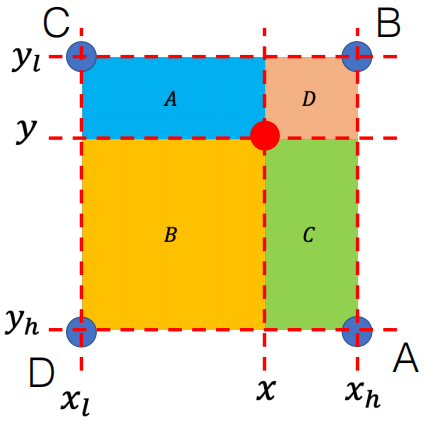
\includegraphics[scale=1.2]{双线性插值.png}
    \caption{双线性插值}
    \label{双线性插值}
\end{wrapfigure}
\begin{equation*}
    f(x^*, y^*) = S_Af(A)+S_Bf(B)+S_Cf(C)+S_Df(D).
\end{equation*}}
\vspace{2cm}
\subsection{Gauss一阶微分的图像梯度}

二维Gauss函数表示如下
\[G_{\sigma}(x, y)=\frac{1}{2\pi \sigma^2}e^{-\frac{x^2+y^2}{2\sigma^2}}\]

对其计算 \(x, y\) 方向上偏导得
\[\frac{\partial G_{\sigma}(x, y)}{\partial x}=-\frac{x}{2\pi \sigma^4}e^{-\frac{x^2+y^2}{2\sigma^2}},\quad \frac{\partial G_{\sigma}(x, y)}{\partial y}=-\frac{y}{2\pi \sigma^4}e^{-\frac{x^2+y^2}{2\sigma^2}}\]

再将两种方向偏导对应的高斯偏导核作用在图像上,分别得到图像在两个方向上的偏导,记为
\(f_x, f_y\),于是根据下式可以分别计算出每个像素处梯度的幅度图(范数)和方向图
\[||\nabla f||(m,n) = \sqrt{f_x(m,n)^2+f_y(m,n)^2},\quad \theta(m,n) = \arctan\left(\frac{f_y(m,n)}{f_x(m,n)}\right).\]

\subsection{Canny边缘检测}

Canny边缘检测算法共分为以下三步:

\begin{enumerate}
\def\labelenumi{\arabic{enumi}.}
\item
  \textbf{梯度提取},取方差为 \(\sigma\)
  的Gauss一阶微分核做卷积,得到幅度图和方向图.
\item
  \textbf{非极大值像素梯度抑制}(Non-Maximum Suppression,
  NMS),对每个像素考虑其梯度方向上的两个临近点,利用之前写好的\textbf{双线性插值}获得两点处的梯度值,然后判断中间点的梯度范数大于两端的梯度范数,若大于则保留,反之舍弃(归零).

  具体来讲,设当前像素点为 \(\boldsymbol{q}: (x, y)\), 幅度函数记为
  \(||\nabla f||(x, y)\),\(\boldsymbol{q}\) 点处的梯度方向记为
  \(\theta\),则考虑沿梯度方向上的两点

  \[\boldsymbol{r}:(x+\cos \theta, y+\sin\theta),\quad
  \boldsymbol{p}=(x-\cos\theta, y-\sin\theta)\]

  若
  \(||\nabla f||(\boldsymbol{q}) > \max\{||\nabla f||(\boldsymbol{r}),||\nabla f||(\boldsymbol{p})\}\),则保留该点,否则令
  \(f(\boldsymbol{q}) = 0\).
\item
  \textbf{高低阈值处理,边缘连接},考虑对NMS结果进一步处理,首先设定高低阈值,这里我使用的是按照幅度值的分位数确定阈值,可以根据不同图像进行自适应阈值大小.
  我们称所有幅度值大于高阈值的点为\textbf{高阈值点},所有幅度值大于低阈值的点为\textbf{低阈值点}.
  然后,将高阈值点从大到小进行枚举,每个点使用深度优先搜索查找边缘,假设当前搜索点为
  \(\boldsymbol{x}\),考虑周围八个方向
  \(\boldsymbol{y}_i\),分为以下四种情况:

  \begin{itemize}
  \item
    若 \(\boldsymbol{y}_i\)
    为搜索树上的父节点或上两层节点(这里判断两层是因为从其他结点到达该节点,在八个方向的领域内,最多是通过存在两个祖先节点),则跳过该节点.
  \item
    若存在 \(\boldsymbol{y}_i\) 为高阈值点,则从高阈值中幅度值最大
    \(\boldsymbol{y}_i\) 开始进行搜索,连接
    \((\boldsymbol{x}, \boldsymbol{y}_i)\),并对 \(\boldsymbol{y}_i\)
    进行迭代搜索.
  \item
    若不存在 \(\boldsymbol{y}_i\) 为高阈值点,且存在
    \(\boldsymbol{y}_i\) 为低阈值点,则取低阈值中幅度值最大的
    \(\boldsymbol{y}_i\),连接
    \((\boldsymbol{x}, \boldsymbol{y}_i)\),返回迭代.
  \item
    若无低阈值点,则返回迭代.
  \end{itemize}
\end{enumerate}

为保持边缘的连续性,连接 \((\boldsymbol{x}, \boldsymbol{y}_i)\)
的具体操作为,若 \(\boldsymbol{y}_i\) 是 \(\boldsymbol{x}\)
的正上下左右四个位置时,则直接进行连接,若 \(\boldsymbol{y}_i\) 是
\(\boldsymbol{x}\)
的左上、右上、左下、右下四个位置时,以左上为例,继续判断
\(\boldsymbol{x}\)
的正上和正左两个位置的幅度值,取较大者设定为边界点,并将其加入结点
\(\boldsymbol{y}_i\) 的父节点中,其他方向同理.

最后,将凸出像素点删去,若一个边界点周围的边界点个数 \(\leqslant 1\)
则删去该边界点,可以使最终边缘图像更加平滑.

\subsection{Harris角点检测}
设图像为$I(\cdot\, ;\cdot)$,考虑一个大小为$2k+1\times 2k+1$中心位于$\bd{x}_0\in\R^2$的滑动窗口$W_k(\bd{x}_0)$,任取一个滑动方向$\bd{t}\in\R^2$,定义在$\bd{t}$方向上的\textbf{平方误差和(sum of squared differences, SSD)}为
\begin{equation*}
    E_{\bd{x}_0}(\bd{t}) = \sum_{\bd{x}\in W_k(\bd{x}_0)}\left(I(\bd{x}+\bd{t})-I(\bd{x})\right)^2
\end{equation*}
若$\bd{x}_0$为角点,则$\forall \bd{t}\in\R^2$,$E_{\bd{x}_0}(\bd{t})$都应尽可能大.

记$\bd{t} = (u,v)^T$,由Taylor公式可知
\begin{equation*}
    I(\bd{x} + \bd{t}) = I(\bd{x}) + I_x(\bd{x})u+I_y(\bd{x})v+O(||\bd{t}||_2^2)
\end{equation*}
于是可对$E_{\bd{x}_0}(\bd{t})$进行进一步分解
\begin{align*}
    E_{\bd{x}_0}(\bd{t})\approx&\  \sum_{x\in W_k(\bd{x}_0)}\left(I(\bd{x}) + I_x(\bd{x})u+I_y(\bd{x})v-I(\bd{x})\right)^2\\
    =&\ \sum_{\bd{x}\in W_k(\bd{x}_0)}\left(I_x(\bd{x})u+I_y(\bd{x})v\right)^2.
\end{align*}

更一般的,设图像$I$大小为$M\times N$,记全体像素点集为$D:=[1,M]\times [1,N]\cap \Z^2$,则
\begin{align*}
    E_{\bd{x}_0}(\bd{t})\approx&\ \sum_{\bd{x}\in D}w_{\bd{x}_0}(\bd{x})\left(I_x(\bd{x})u+I_y(\bd{x})v\right)^2\\
    =&\ \sum_{\bd{x}\in D}w_{\bd{x}_0}(\bd{x})I_x^2(\bd{x})u^2+ 2w_{\bd{x}_0}(\bd{x})I_x(\bd{x})I_y(\bd{x})uv+w_{\bd{x}_0}(\bd{x})I_y^2(\bd{x})v^2\\
    =&\ A(\bd{x}_0)u^2+2B(\bd{x}_0)uv+C(\bd{x}_0)v^2.
\end{align*}
其中$w_{\bd{x_0}}(\bd{x}) = \begin{cases}
    1,&\quad \bd{x}\in W_k(\bd{x}_0),\\
    0,&\quad \texttt{otherwise}.
\end{cases}$为$W_k(\bd{x}_0)$的示性函数,\add 为使其变化更平滑,可取$w_{\bd{x}_0}$为中心在$\bd{x}_0$大小为$2k+1\times 2k+1$的Gauss核,上式中$A,B,C$定义如下,分别表示将核$w$作用在$I_x^2,\ I_xI_y,\ I_y^2$图像上得到的结果
\begin{equation*}
A(\bd{x_0}) = \sum_{x\in D}w_{\bd{x}_0}(\bd{x})I_x^2(\bd{x}),\ B(\bd{x_0}) = \sum_{x\in D}w_{\bd{x}_0}(\bd{x})I_x(\bd{x})I_y(\bd{x}),\ C(\bd{x_0}) = \sum_{x\in D}w_{\bd{x}_0}(\bd{x})I_y^2(\bd{x}).
\end{equation*}
进一步,可使用二次型矩阵表出
\begin{equation*}
    E_{\bd{x}_0}(\bd{t}) = \bd{t}^TM_{\bd{x}_0}\bd{t},\quad \text{其中 }M_{\bd{x}_0}=\left[\begin{matrix}
        A(\bd{x_0})&B(\bd{x}_0)\\
        B(\bd{x_0})&C(\bd{x}_0)\\
    \end{matrix}\right]
\end{equation*}
称$M_{\bd{x}_0}$为图像在$\bd{x}_0$处的二阶矩矩阵.

假设$M_{\bd{x}_0}$的秩为$2$,则$M_{\bd{x}_0}$存在$2$个特征值,记其中较大者为$\lambda_{max}$,较小者为$\lambda_{min}$,对应的特征向量分别为$\bd{x}_{max},\ \bd{x}_{min}$,由特征向量定义可知,$M_{\bd{x}_0}\bd{x}_{max} = \lambda_{max}\bd{x}_{max}$说明窗口$W_k(\bd{x}_0)$在沿着$\bd{x}_{max}$方向上移动单位长度,$E_{\bd{x_0}}(\bd{t})$可达到最大值. 下面对$\lambda$的大小进行分类讨论

1. 当$\lambda_{max}$较小时,$E_{\bd{x_0}}(\bd{t})$沿各个方向变化都较小,则$\bd{x}_0$处于图像内部平滑区域.

2. 当$\lambda_{max}$较大且$\lambda_{max}\approx\lambda_{min}$时,$E_{\bd{x_0}}(\bd{t})$沿各个方向变化都较大,则$\bd{x}_0$是角点.

3. 当$\lambda_{max}$较大且$\lambda_{max}>>\lambda_{min}$时,$E_{\bd{x_0}}(\bd{t})$仅沿$\bd{x}_{max}$方向变化较大,则$\bd{x}_0$是边界点.

通过引入\textbf{角点响应函数(Corner response function)}用于判断角点
\begin{align*}
    R(\bd{x}_0) =&\ \det(M_{\bd{x}_0}) - \alpha\cdot\text{trace}(M_{\bd{x}_0})^2 = \lambda_1\lambda_2 - \alpha(\lambda_1+\lambda_2)^2\\
    =&\ A(\bd{x_0})C(\bd{x_0}) - B^2(\bd{x_0}) - \alpha(A(\bd{x_0})+C(\bd{x_0}))
\end{align*}
其中$\alpha\in[0.04,0.06]$为超参数. 当$R(\bd{x}_0)$大于设定阈值时,则判定$\bd{x}_0$为角点.

最后,再使用\textbf{非局部极大值抑制(Non-maxima suppression, NMS)},若$\bd{x}_0$是其邻域内的最大值,则对其进行保留,否则删去该点. 通过设定邻域大小,可对角点密度进行调整.

整个Harris角点检测算法中,总共存在4个超参数,分别为窗口大小$k$,响应函数中$\alpha$,响应阈值和NMS邻域大小.

\clearpage
\section{实验步骤与结果分析}
\subsection{完成上次未完成的填充操作}
\begin{figure}[htbp]
    \centering
    \hspace*{-1.5cm}
    \includegraphics[scale=0.4]{D:/yy/Documents/GitHub/CVPR_homeworks/code/hw2/CVPR2_note.figure/填充操作1.png}
    \caption{填充操作1}
\end{figure}
\begin{figure}[htbp]
    \centering
    \hspace*{-1.5cm}
    \includegraphics[scale=0.4]{D:/yy/Documents/GitHub/CVPR_homeworks/code/hw2/CVPR2_note.figure/填充操作2.png}
    \caption{填充操作2}
\end{figure}
\subsection{几何变换实验(5种变换)}
图像坐标系默认是按照左上角为原点,纵轴向下为 \(x\) 轴正方向,横轴向右为
\(y\)
轴正方向,为便于输出查看,变化后的图像保持与原图像相同的大小,但这样就会发生图像大部分空白,所以需要使用平移矩阵将变化后的图像中心保持在输出框的中心,具体来说,假设图像大小为
\(N\times M\),几何变换为 \(T\),记图像中心点为
\(\boldsymbol{x}_{mid} = (N/2,M/2)\) ,则考虑平移向量和对应的平移矩阵为

\[\boldsymbol{t} = \boldsymbol{x}_{mid} - T\boldsymbol{x}_{mid},\quad T_{translation}=\left[\begin{matrix}1&0&t_1\\ 0&1&t_2\\0&0&1\end{matrix}\right]\]

最后将$T\times T_{translation}$作用在原图上即可获得中心化图片,为了保证输出效果,除平移操作和旋转操作外,其他操作都进行平移,向前变换会很多空洞,而反向变换的效果好得多. 实验效果如图\ref{fig-0},图\ref{fig-1}所示.

\begin{figure}[htbp]
    \centering
    \hspace*{-1.5cm}
    \includegraphics[scale=0.6]{D:/yy/Documents/GitHub/CVPR_homeworks/code/hw2/CVPR2_note.figure/向前变换.png}
    \caption{向前变换\label{fig-0}}
\end{figure}
\begin{figure}[htbp]
    \centering
    \hspace*{-1.5cm}
    \includegraphics[scale=0.6]{D:/yy/Documents/GitHub/CVPR_homeworks/code/hw2/CVPR2_note.figure/几何变换实验.png}
    \caption{反向变换,几何变换实验\label{fig-1}}
\end{figure}

\subsection{Gauss金字塔和Laplace金字塔}

Gauss金字塔:使用Gauss核与图像做卷积,设定Gauss核移动步长为stride=2,于是每次可将整个图像缩小
\(1/4\) 倍.

在使用matplotlib进行绘图时,由于将图像同时输出到同一个画板上时,其会自动将子图进行放大,以保持相同的图像大小,所以为了输出图像金字塔的效果,需自行设定每个子图的坐标,四种距离参数包括:左侧,底部,横向,竖向. 实验效果如图\ref{fig-2}所示.

\begin{figure}[htbp]
    \centering
    \includegraphics[scale=0.4]{D:/yy/Documents/GitHub/CVPR_homeworks/code/hw2/CVPR2_note.figure/下采样缩小结果.png}
    \caption{Gauss金字塔\label{fig-2}}
\end{figure}

在进行上采样放大图像过程中,由于要对原图进行0填充补其奇数行与奇数列,然后再用大小为5的Gauss核做卷积,这样会是的图像的整体亮度偏低,最后通过对全体像素乘
\(4\) 来提高亮度(经过尝试,感觉这个大小和原图亮度最接近,如图\ref{fig-3}所示).
在这里进行Gauss做卷积的过程中,我尝试了 \(4\)
中不同的边界填充方法,其中边界镜像的效果最好,所以在下述上采样操作中都是用该边界填充方法.

\begin{figure}[htbp]
    \centering
    \hspace*{-1cm}
    \includegraphics[scale=0.4]{D:/yy/Documents/GitHub/CVPR_homeworks/code/hw2/CVPR2_note.figure/上采用使用不同边界填充.png}
    \caption{使用不同边界填充\label{fig-3}}
\end{figure}

\begin{figure}[htbp]
    \centering
    \subfigure[上采样金字塔]  % 子图的标题
    {
        % 如果一行放三个图改成0.3\linewidth即可
        \hspace*{-3cm}\begin{minipage}[b]{.6\linewidth}  % 0.45排版行距, 即一行放2个图, 一行放不下就换行
            \centering
            \includegraphics[scale=0.4]{D:/yy/Documents/GitHub/CVPR_homeworks/code/hw2/CVPR2_note.figure/上采样放大结果.png}
        \end{minipage}
    }
    \subfigure[Laplace金字塔]
    {
        \begin{minipage}[b]{.35\linewidth}
            \centering
            \includegraphics[scale=0.4]{D:/yy/Documents/GitHub/CVPR_homeworks/code/hw2/CVPR2_note.figure/Laplace金字塔.png}
        \end{minipage}
    }
\end{figure}

下面讨论低通滤波和抽样频率的关系,由Shannon-Nyquist定理可知,采样频率应至少大于最大频率的2倍以上才不会发生图像像素混淆.
图像使用的是“黄鹤楼”,因为该建筑上具有非常多的细节纹理,从上次作业Fourier变换结果来看,该图具有较高的频率,像素重叠现象更为明显.
下图分布以直接进行下采样和做Gauss模糊以后再进行采样进行比较,体现Gauss模糊确实能有效降低图像的频率.

\begin{figure}[htbp]
    \centering
    \hspace*{-1.5cm}
    \includegraphics[scale=0.4]{D:/yy/Documents/GitHub/CVPR_homeworks/code/hw2/CVPR2_note.figure/直接进行采样.png}
    \caption{直接进行采样\label{fig-4}}
\end{figure}

\begin{figure}[htbp]
    \centering
    \hspace*{-1.5cm}
    \includegraphics[scale=0.4]{D:/yy/Documents/GitHub/CVPR_homeworks/code/hw2/CVPR2_note.figure/Gauss模糊以后进行下采样.png}
    \caption{使用Gauss模糊后进行采样\label{fig-5}}
\end{figure}

\clearpage
\subsection{Gauss一阶微分的图像梯度}
\(\sigma = 3\),大小为\(13\times 13\) 的高斯核分别在 \(x,y\)
轴方向上的偏导如下图所示(这里以图像纵轴向下为 \(x\) 正方向,横轴向右为
\(y\) 轴正方向).

\textbf{注}:此处Gauss一阶微分核无需再进行归一化处理.

\begin{figure}[htbp]
    \centering
    \includegraphics[scale=0.4]{D:/yy/Documents/GitHub/CVPR_homeworks/code/hw2/CVPR2_note.figure/两种Gauss一阶微分核.png}
    \caption{两种Gauss一阶微分核\label{fig-6}}
\end{figure}

实际操作中,要显示幅度谱需要使用\textbf{线性正规化方法},而显示方向图要使用\textbf{截断正规化方法},下图实验了将
\(\sigma=0.5, 1, 5\) 分别作用在图像上,得到梯度的幅度图和方向图

\begin{figure}[htbp]
    \centering
    \hspace*{-1.5cm}
    \includegraphics[scale=0.4]{D:/yy/Documents/GitHub/CVPR_homeworks/code/hw2/CVPR2_note.figure/梯度的幅度图和方向图.png}
    \caption{幅度图和方向图\label{fig-7}}
\end{figure}

从中可以看出,高斯核方差越大,幅度图中边缘提取更加多,但是边缘厚度太大,导致后续进一步处理困难,所以选取适合的方差十分关键,从图中可看出
\(\sigma=2\) 时提取效果较好.

\subsection{Canny边缘检测}
在NMS过程中,发现梯度的幅度图均值仅有
\(0.00858\),为了使得进行线性插值时便于加权求和,对幅度谱先均值提升到1.
下图所展示的NMS过程,NMS过程共计删除 \(38945\) 个像素点,占比
\(14.856339\%\),设定低阈值为分位数 \(50\%\) 的像素值,高阈值为分位数
\(92\%\) 的像素值,边缘连接过程共计连接 \(14756\) 个像素点,占比
\(5.628967\%\).

超参数对边缘检测结果的影响:$\sigma$越大图像更为模糊,梯度的变化更为平滑,导致边缘更粗,不能很好的确定边缘位置. 高阈值与低阈值使用分位数进行确定,高阈值一般取为$95\%,92\%$,若取值较低,则会导致将较多非边缘边加入,效果变差. 而低阈值的取值$80\%$与$50\%$的区别其实不是非常大,因为有边缘连接算法保证边缘的连接不会因为低阈值的增大而导致边缘变粗.

所以决定最终检测效果的主要是确定$\sigma$和高阈值的分位数,还有边缘连接算法.

\begin{figure}[htbp]
    \centering
    \includegraphics[scale=0.6]{D:/yy/Documents/GitHub/CVPR_homeworks/code/hw2/CVPR2_note.figure/Canny边缘检测.png}
    \caption{边缘检测\label{fig-8}}
\end{figure}
\vspace*{-1cm}
\subsubsection{Harris角点检测}
通过调整不同的窗口大小,旋转角度和亮度,角点检测结果如图\ref{fig-10}和图\ref{fig-11}所示,该结果表明,窗口大小越小,能检测出的角点个数越多密度越大,因为小窗口中梯度变化会更加明显,而大窗口中梯度变化更为平均,只有梯度变化明显的点才会被识别出来.

\begin{figure}[htbp]
    \centering
    \includegraphics[scale=0.5]{D:/yy/Documents/GitHub/CVPR_homeworks/code/hw2/CVPR2_note.figure/角点检测1.png}
    \caption{角点检测1\label{fig-9}}
\end{figure}

\begin{figure}[htbp]
    \centering
    \includegraphics[scale=1]{D:/yy/Documents/GitHub/CVPR_homeworks/code/hw2/CVPR2_note.figure/角点检测31.png}
    \caption{角点检测小窗口\label{fig-10}}
\end{figure}

\begin{figure}[htbp]
    \centering
    \includegraphics[scale=1]{D:/yy/Documents/GitHub/CVPR_homeworks/code/hw2/CVPR2_note.figure/角点检测32.png}
    \caption{角点检测大窗口\label{fig-11}}
\end{figure}
\vspace*{-1cm}
\section{结论与讨论}
本次实验进一步学习了更多的图像特征提取操作,对图像处理代码库功能进行完善. 在Canny算法的边缘连接部分使用了较为复杂的贪心方法,能有效的降低了边缘的厚度,但仍未达到OpenCV的效果,主要是边缘处不够光滑,有待进一步改进.

完整代码请见:\url{https://github.com/wty-yy/CVPR_homeworks/tree/master/code/hw2}.

\end{document}

\iffalse
%%%% 表格模板 %%%%
\renewcommand\arraystretch{0.8} % 设置表格高度为原来的0.8倍
\begin{table}[!htbp] % table标准
    \centering % 表格居中
    \begin{tabular}{p{1cm}<{\centering}p{1cm}<{\centering}p{3cm}<{\centering}p{5cm}<{\centering}} % 设置表格宽度
    %\begin{tabular}{cccc}
        \toprule
        $x_i$ & $f[x_1]$ & $f[x_i, x_{i+1}]$ & $f[x_i, x_{i+1}, x_{i+2}]$ \\
        \midrule
        $x_0$ & $f(x_0)$ &                  &                          \\
        $x_0$ & $f(x_0)$ & $f'(x_0)$        &                          \\
        $x_0$ & $f(x_1)$ & $\frac{f(x_1)-f(x_0)}{x_1-x_0}$ & $\frac{f(x_1)-f(x_0)}{(x_1-x_0)^2}-\frac{f'(x_0)}{x_1-x_0}$\\
        \bottomrule
    \end{tabular}
\end{table}

%%%% 文字环绕图片, 标题加注释 %%%%
{ % 一般将文字环绕部分的图和文字, 用大括号括起来, 避免对文字外的格式发生影响
\begin{wrapfigure}[13]{r}{.5\linewidth} % 文字环绕行数为13行, 图片靠右 (l为靠左), 图片占0.5的行宽
    \centering
    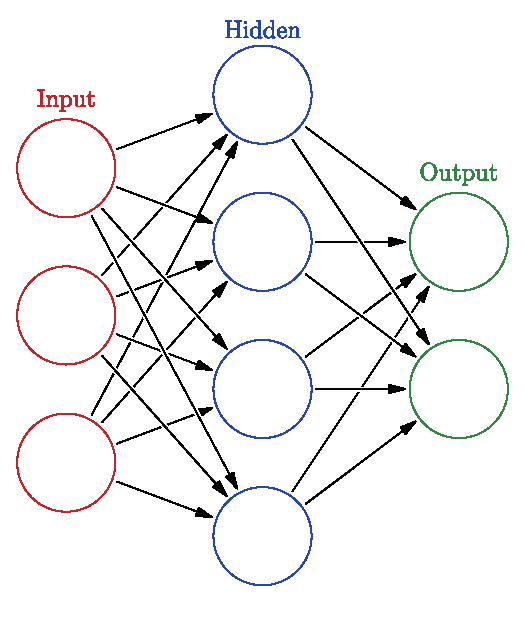
\includegraphics[scale=0.7]{neural_network.eps} % scale=0.7按比例缩放70%
    \caption{神经网络结构\protect\footnotemark[1]} % 记得加\protect, 设置1号脚标
    \label{figure-神经网络结构}
\end{wrapfigure}
\footnotetext[1]{图片来源: \url{https://en.wikipedia.org/wiki/File:Colored_neural_network.svg}}
文字文字
}

%%%% 普通图片, 标题加注释 %%%%
\begin{figure}[htbp] % h: 当前位置, t: 顶部, b: 底部, p: 浮动页, 这样组合指的是使用这个顺序进行排版
    \centering
    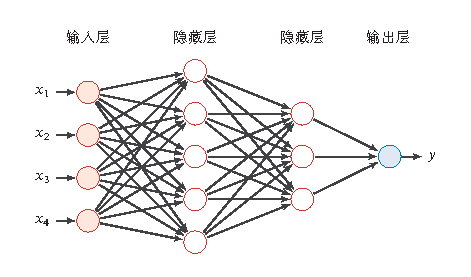
\includegraphics[scale=0.5]{前馈神经网络.eps}
    \caption{前馈神经网络\protect\footnotemark[1]}
    \label{figue-前馈神经网络}
\end{figure}
\footnotetext[1]{图片来源: 邱锡鹏, 神经网络与深度学习 \cite{ref-qxp}, 第92页}

%%%% 多组图 %%%%
    \begin{figure}[htbp]
        \centering
        \subfigure[迭代1次]  % 子图的标题
        {
            % 如果一行放三个图改成0.3\linewidth即可
            \begin{minipage}[b]{.45\linewidth}  % 0.45排版行距, 即一行放2个图, 一行放不下就换行
                \centering
                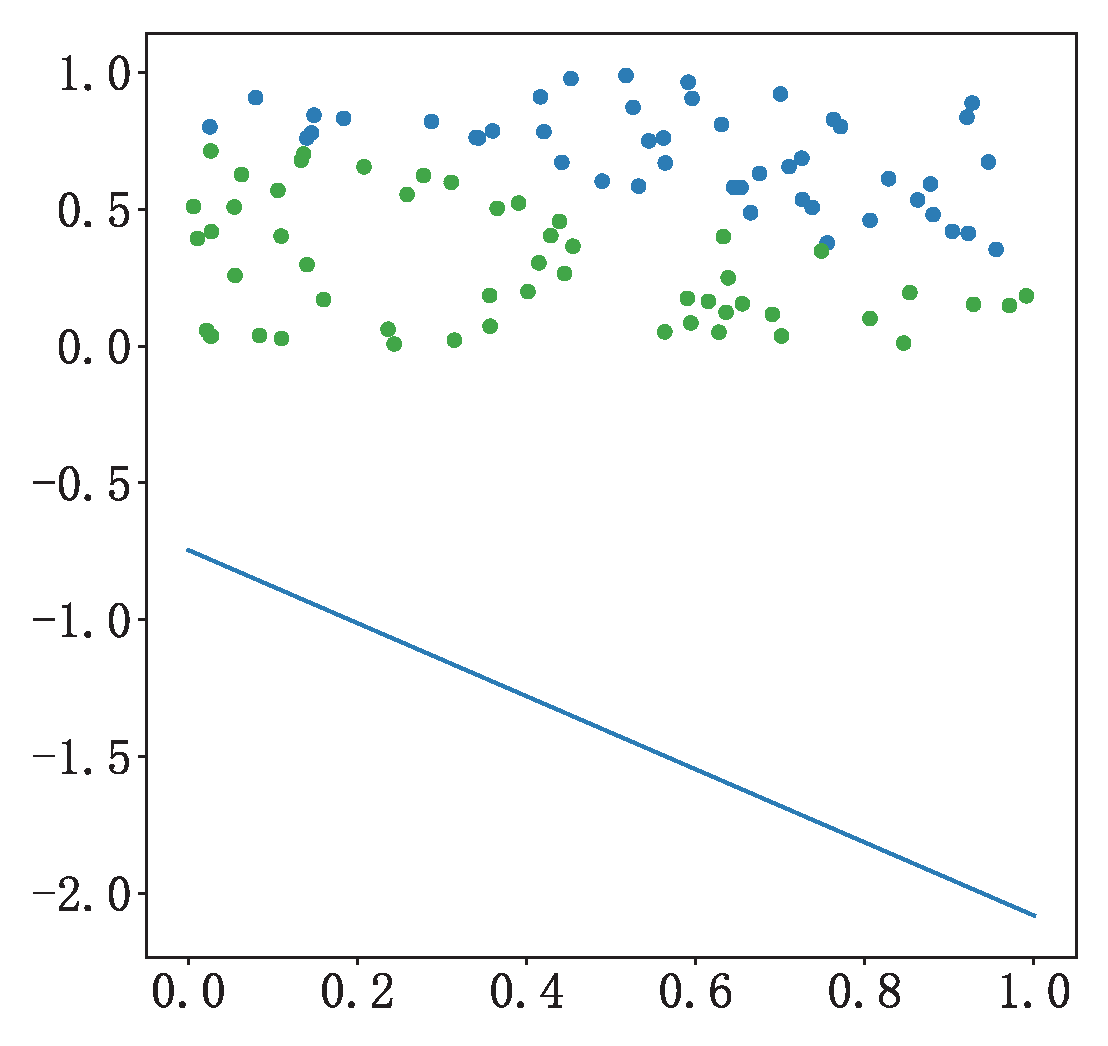
\includegraphics[scale=0.35]{1.eps}
            \end{minipage}
        }
        \subfigure[迭代100次]
        {
            \begin{minipage}[b]{.45\linewidth}
                \centering
                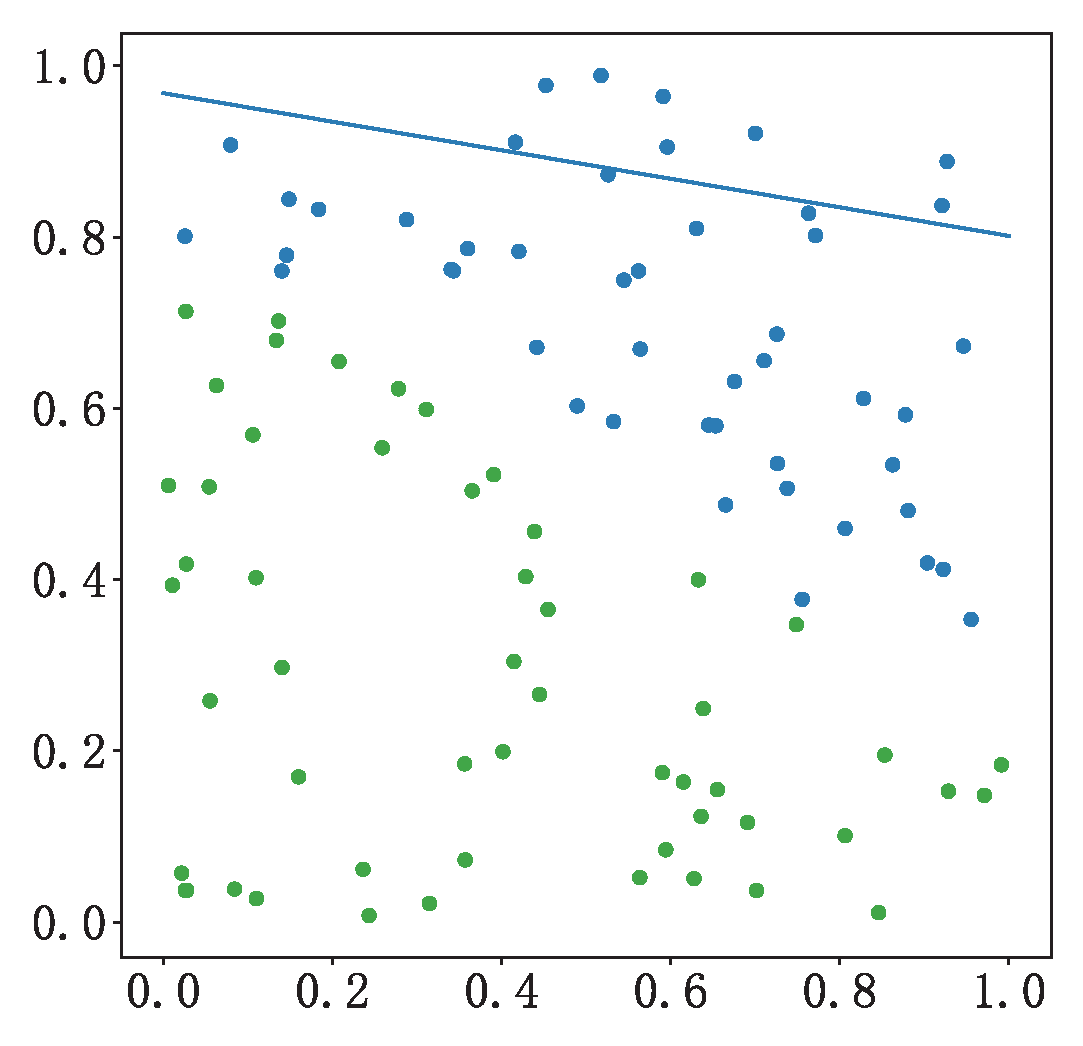
\includegraphics[scale=0.35]{100.eps}
            \end{minipage}
        }
        \subfigure[迭代500次]
        {
            \begin{minipage}[b]{.45\linewidth}
                \centering
                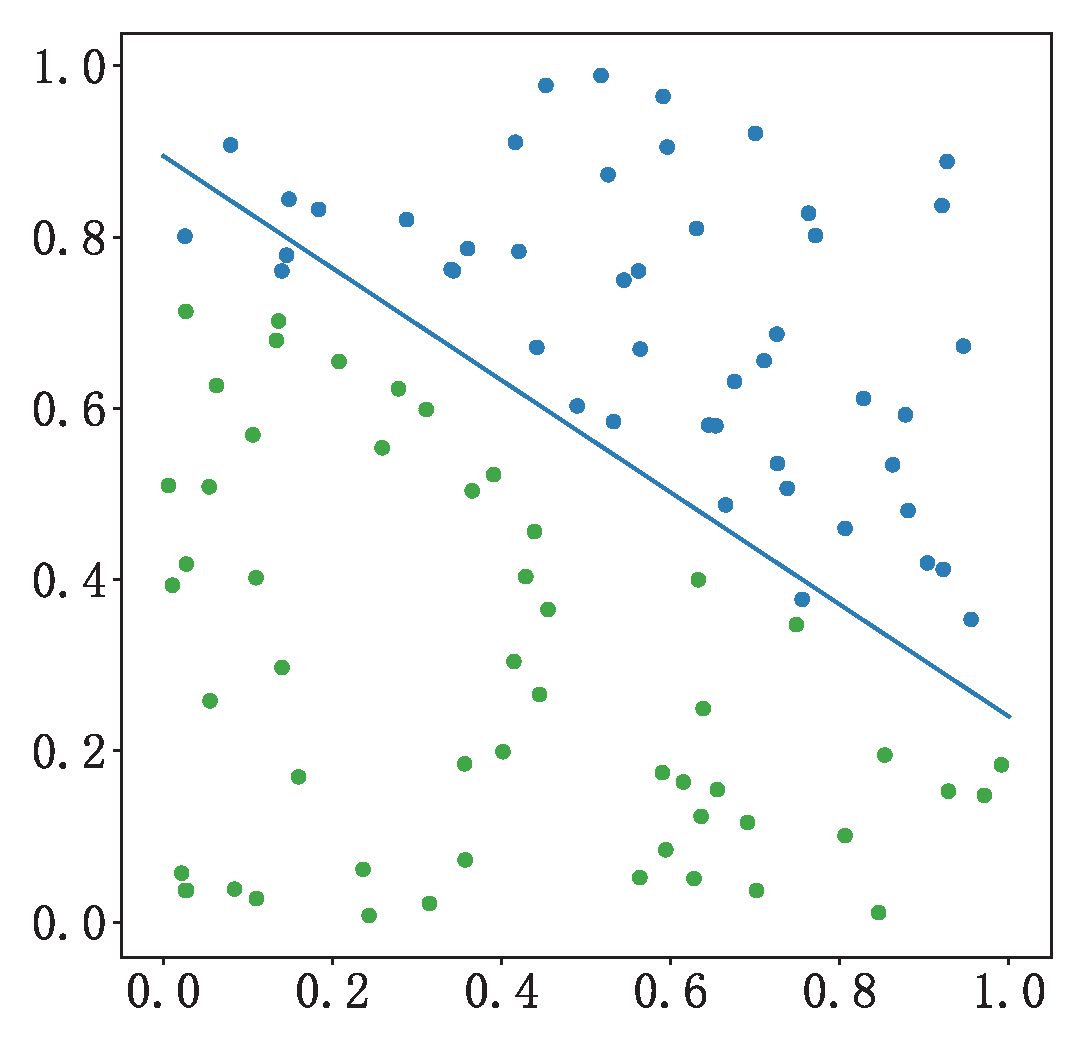
\includegraphics[scale=0.35]{500.eps}
            \end{minipage}
        }
        \subfigure[迭代2000次]
        {
            \begin{minipage}[b]{.45\linewidth}
                \centering
                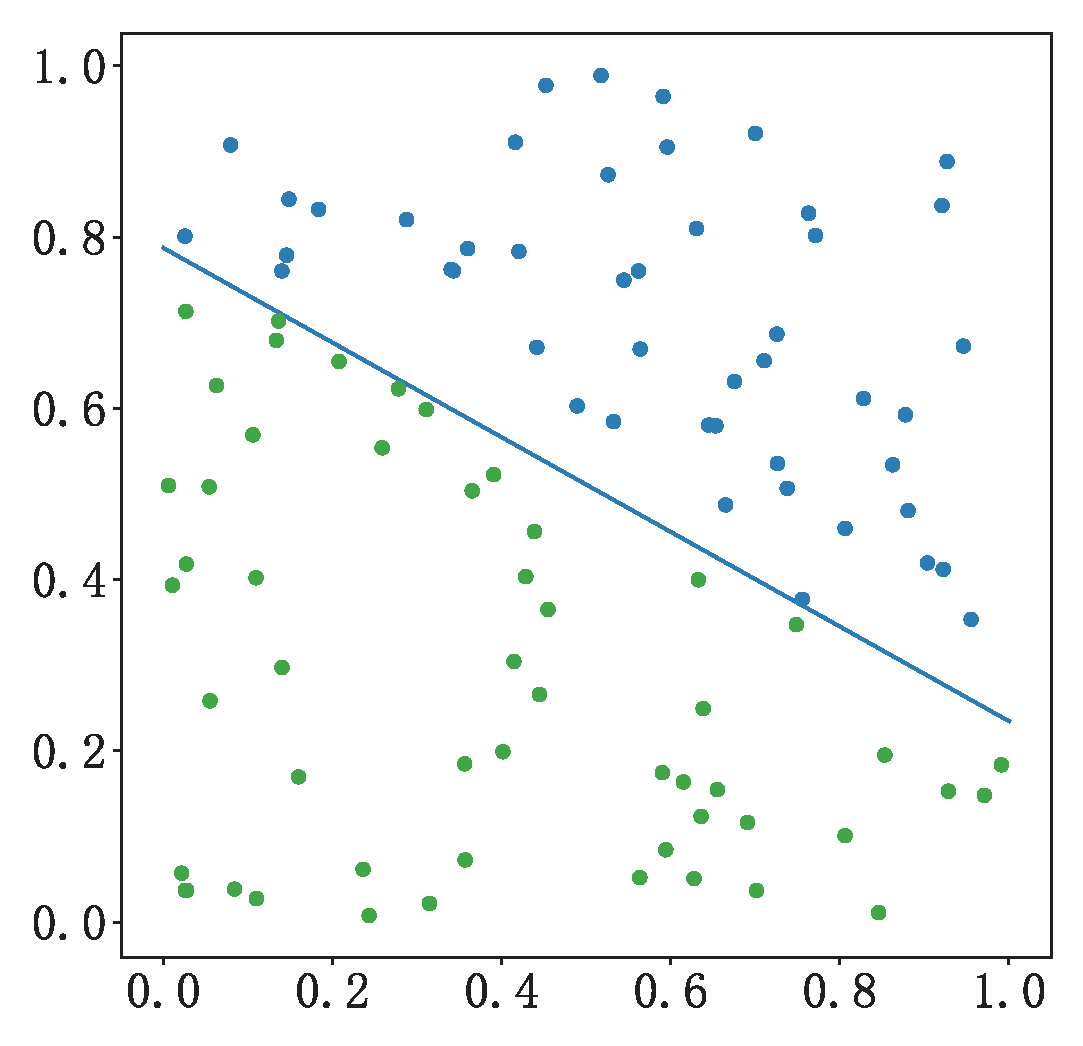
\includegraphics[scale=0.35]{2000.eps}
            \end{minipage}
        }
        \caption{迭代过程图}
        \label{figure-迭代过程图}
    \end{figure}
\fi
